\chapter{Incremental view synchronization}
\label{chap:transform}

Complex industrial toolchains used for the model-based design of safety-critical cyber-physical systems frequently depend on various models on different levels of abstraction where abstract models are derived by model transformations. The derived models are often \emph{views}, which aim to focus attention from a given \emph{viewpoint} such that details relevant to a specific group of stakeholders are retained~\citep{Bruneliere17survey}. The views contain information that is related to and coming from other models, which can also be themselves other views. Incremental small-step execution of model transformations aids in reducing the computations costs of view maintenance~\citep{Varro15styles}.

In this chapter we propose a means to assemble formal stochastic models from domain models by model transformation. The resulting analysis model is a \emph{view} of the engineering model from a \emph{reliability} or \emph{performability} viewpoint. The transformation should be \circled{1}~\emph{parametric} in the sense that the source metamodel, the transformation rules and the analysis model fragments that are instantiated may be specified by the user. In addition, stochastic Petri nets produced by the transformation should be \circled{2}~\emph{compatible with external analysis tools.} As a key to interpret analysis results of the derived stochastic models automatically, the transformation should ensure \circled{3}~\emph{end-to-end traceability} between source model elements and the quantitative aspects of the stochastic model. Lastly, to support efficient mapping of constantly changing design candidates in design-space exploration, the transformation should be \circled{4}~\emph{executed incrementally} driven by change notifications of the source model.

Existing transformation languages, such as \textabbr{ATL}~\citep{Jouault08atl}, \mixedabbr{QVT}r~\citep[Chapter~7]{OMG16qvt} or \textabbr{VIATRA} Views~\citep{Debreceni14viewmodel} can describe mappings between instances of arbitrary metamodels; therefore they satisfy the requirement of \circled{1}~user configurability. These language require the specification of the results of the transformation at the low level of individual model objects and links. While creating single objects at once is satisfactory for views that aim to create \emph{abstractions} of the source model, automatic derivation of stochastic models is closer to \emph{compilation}. The result of mapping even just one source element may have a complicated result, such as a collection of Petri net places, transitions and expressions trees describing quantitative aspects of the model. Hence we propose a transformation specification language tightly integrated with \textAbbr{RGSPN}s introduced in \cref{chap:rgspn} as an alternative to general-purpose transformation languages for stochastic model creation.

The left side of the transformation rules are graph patterns which select the parts of the source model to be mapped. On the right side, the transformation results are specified as \emph{\textabbr{RGSPN} modules}, which are \textAbbr{RGSPN} model fragments. The typing discipline from \vref{dfn:rgspn:well-typed} is extended to transformation rules to aid in catching bugs.

In current analysis tools, there is little support for reference symbols, variables and collections introduced in \textAbbr{RGSPN}s. To \circled{2}~ensure compatbility, a \emph{inlining} step is also incorporated into the transformation chain. The inlining \emph{concretizes} the \emph{abstract} \textabbr{RGSPN} constructed according to the user-provided view specification and yields a \emph{concrete} \textabbr{RGSPN}, that contains no references, collections or references to variables. Variable symbols are kept so that they can exported to the analysis tool as stochastic metrics to be computed or as queries to be answered. Matching of the queries to source model concepts is provided by \circled{3}~traceability relations that are maintained implicitly, i.e.~without additional user intervention.

The \circled{4}~incremental execution of the transformation is ensured by the use of an incremental graph query engine~\citep{Ujhelyi15incquery} and a reactive model transformation platform~\citep{Bergmann15viatra}. If a step in the transformation chain cannot be executed due to a malformed input model the effects of the transformation are \emph{delayed} until the issue is resolved. Upon delaying, an error marker is generated that is removed when the transformation can resume successfully.

After briefly reviewing related work we describe the proposed transformation chains, as well as its specification language and semantics. Then the instantiation of \textabbr{RGSPN} modules is discussed, finally followed by the details of the concretization transformation and its handling of inconsistencies by the means of delayed execution.

\section{Related work: view synchronization for formal models}
\label{chap:transform:relwork}

\subsection{Incremental transformation languages}

\todo*{}

\subsection{Transformation languages for stochastic models}

\todo*{}

\section{Overview of the transformation engine}
\label{chap:transfrom:specify}

\begin{figure}
  \centering
  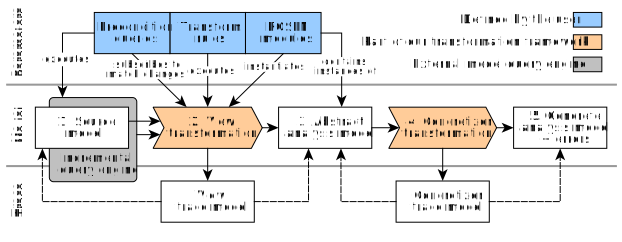
\includegraphics[scale=0.9]{figures/transformation_chain}
  \caption{Overview of the transformation chain.}
  \label{fig:transform:overview}
\end{figure}

\subsection{Transformation specifications}

\begin{table}%
  \caption{Transformation specification for dining philosophers domain models.}%
  \lstset{
    basicstyle={\ttfamily\small},
    columns=fixed,numbers=none,
    aboveskip=0pt,belowskip=-1.2\baselineskip,
    language=ecore2pn
  }%
  \centering
  \begin{tabular}{@{}>{\centering\arraybackslash}m{0.20\textwidth}@{}m{0.42\textwidth}@{}>{\centering\arraybackslash}m{0.38\textwidth}@{}}
    \toprule
    \multicolumn{1}{@{}c}{Precondition} & \multicolumn{1}{c}{Transformation rule} &
    \multicolumn{1}{c@{}}{\textabbr{RGSPN} module} \\
    \midrule
    & \begin{lstlisting}
features {
\end{lstlisting} & \\
    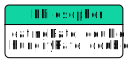
\includegraphics[scale=0.8]{figures/phil_class}& \begin{lstlisting}
  Philosopher {
    param eatingRate
  }
\end{lstlisting} &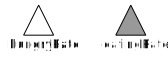
\includegraphics[scale=0.8]{figures/phil_features}\\
  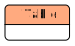
\includegraphics[scale=0.8]{figures/table_class}& \begin{lstlisting}
  Table {
    derived prop double
        ^totalThinkingTime^
  }
\end{lstlisting} &
\includegraphics[scale=0.8]{figures/table_features}\\
  & \begin{lstlisting}
}
\end{lstlisting} & \\
  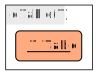
\includegraphics[scale=0.8]{figures/q_table_pattern}& \begin{lstlisting}
mapping qTable(T)
    => TableMod TM {
  T.^totalThinkingTime^
      := TM.totalThinkingTime
}
\end{lstlisting} &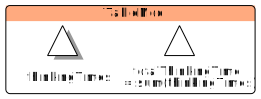
\includegraphics[scale=0.8]{figures/table_module}\\[-0.2ex]
  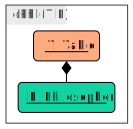
\includegraphics[scale=0.8]{figures/q_phil_pattern}& \begin{lstlisting}
mapping qPhil(T, P)
    => PhilMod PM {
  lookup qTable(T) => TM
  PM.^hungryRate^ := P.hungryRate
  PM.^eatingRate^ := P.eatingRate
  TM.^thinkingTimes^
      += PM.thinkingTime
}
\end{lstlisting} &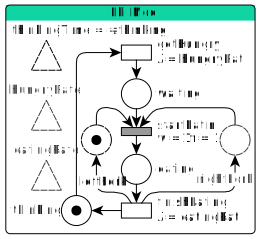
\includegraphics[scale=0.8]{figures/phil_module}\\[-2ex]
  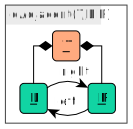
\includegraphics[scale=0.8]{figures/q_adjacent_pattern}& \begin{lstlisting}
mapping qAdjacent(T, L, R) {
  lookup qPhil(T, L) => PM1
  lookup qPhil(T, R) => PM2
  PM2.^leftFork^ := PM1.rightFork
}
\end{lstlisting} &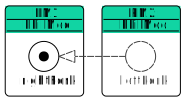
\includegraphics[scale=0.8]{figures/adjacent_phils_module}\\
    \bottomrule
  \end{tabular}
\end{table}

\section{Generic view transformation to stochastic Petri nets}
\label{chap:transform:view}

\section{Stochastic Petri net concretization}
\label{chap:transform:concretizer}